\section{Profiling the \acs{MPM} and \acs{NLP}}
\label{sec:profiling}
The routine described for \ac{FID} estimation involves operations which can be
computationally demanding, with those demands increasing with the number of
points in the \ac{FID}, as well as the number of oscillators in the model. This
is the case both in terms of the amount of work
done by the \ac{CPU}, and the amount of \ac{RAM} needed to store all the
required information as the routine runs. For the \ac{MPM}, the most
demanding aspect is \ac{SVD} calculations while for numerical optimisation, it
is generation of the Hessian matrix at each iteration. Detailed accounts of the
computational complexity of the \ac{MPM} and \ac{MMEMPM} have been
presented\cite{Hua1992,Chen2007}.  However, it is useful to consider what the
actual ``wall-clock times'' of these routines are on a modern computer. A lot of
accounts on the \ac{MPM} are from decades before this work, and so the
time required for the routine to run will have decreased a lot thanks to
improvements in processing power. For example, the account by Pines a co-workers
from 1997 outlining the \ac{ITMPM} states that a signal comprising $1024$
points would take about
\qty{4.5}{\minute} to be processed by the \ac{MDL} and \ac{MPM}, using a
\qty{100}{\mega\hertz} \ac{CPU}\cite{Lin1997}. On the system used for all
results generated for this work (see \cref{rem:workstation}) an
equivalent computation takes about \qty{100}{\milli\second}.
\begin{remark}
    \label{rem:workstation}
    All results generated in this work were acquired using a workstation
    featuring a Intel\textregistered\ Core\texttrademark\ i9-10900X CPU @
    \qty{3.7}{\giga\hertz}, and \qty{32}{\gibi\byte} of RAM.
\end{remark}

\subsection{\acs{1D} \acs{MPM}}
\begin{figure}
    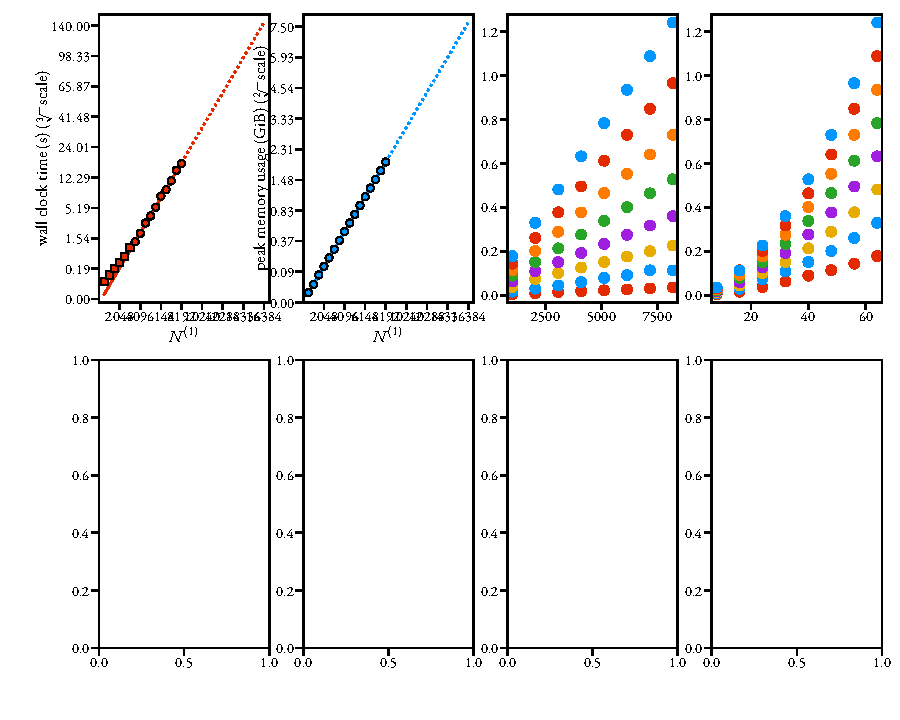
\includegraphics{timings/timings.pdf}
    \caption[
        Profiles outlining the computation times and peak memory consumption of
        the \acs{MPM} and for Hessian construction.
    ]
    {
        Profiles outlining the computation times and peak memory consumption of
        the \acs{MPM} and for Hessian construction.
        \textbf{a.} Wall clock time to compute the \ac{MPM} of \iac{FID}
        with 10 signals, as a function of number of points. Plotted alongside
        the times measured for each $N$ is a cubic fit of the circular points
        (solid: interpolation, dotted: extrapolation).
        \textbf{b.} Peak memory consumption in performing the \ac{MPM}, along
        with a quadratic fit.
        \note{TODO: 1D Hessian: variable M and N, MMEMPM, wall clock and
        memory, 2D Hessian: variable M and product of $\None \Ntwo$.}
    }
    \label{fig:profiling}
\end{figure}

A series of \acp{FID} were constructed with a variable number of time-points
$N \in \lbrace 512k \hspace*{2pt} \vert \hspace*{2pt} k \in \lbrace 1, 2,
\cdots, 16 \rbrace \rbrace$. For each \ac{FID}, the \ac{MPM} was performed 5
times, with a pencil parameter $L = \lfloor \nicefrac{N}{3} \rfloor$.
A \textsc{Python} implementation of the \ac{MPM} was timed using a line
profiler, which outputs the amount of time spent running the code on each line of a
given script\footnote{
    The line profiler used is accessible via:
    \url{https://github.com/pyutils/line_profiler}.
}. The mean complete time to run the \ac{MPM} is plotted as a
function
of $N$ in panel a of \cref{fig:profiling}, where it can be seen that for
sufficiently large $N$ the \ac{MPM} is computed in approximately
$\mathcal{O}({N}^3)$ time. This is due to the most time-consuming aspect of the
\ac{MPM} being the computation of the \ac{SVD} of $\Hy$, whose size is
approximately $\tfrac{2N}{3} \times \tfrac{N}{3}$\footnote{
    The time complexity for the \ac{SVD} of generic a $M \times N$ matrix is
    $\mathcal{O}(\operatorname{min}(M, N)^2 \cdot \operatorname{max}(M, N))$
}. For small values of $N$ (i.e. the square points in the plot), a deviation
away from a cubic relationship is observed. This is since the computation of
the complex amplitudes in accordance with \cref{eq:comp-amps} has a
comparatively significant run time\footnote{
    For a $512$ point signal, the \ac{SVD} of $\Hy$ took up roughly 80\% of the
    complete run time, while the computation of the complex amplitudes took up
    roughly 20\%. For a 8192 point signal, these percentages had changed to
    $>\!99\%$ and $<\!1\%$, respectively.
}. The figure shows the fit of a cubic function, of the form $aN^3 + b$, to the
circular points, corresponding to values of $N$ in the ``cubic regime''.
This function has been extrapolated to 16k points, to give an idea of the
required run-time over a wide range of $N$ (of course, the run time will vary
depending on the hardware used).

To assess the effect of \ac{FID} size on the space complexity of the \ac{MPM},
the routine was run again for each $N$ defined, with a memory profiler
analysing the amount of \ac{RAM} used with time\footnote{
 The memory profiler used is accessible via:
 \url{https://github.com/pythonprofilers/memory_profiler}.
}. The peak \ac{RAM} consumption is plotted in panel b of \cref{fig:profiling}.
A clear quadratic dependence of consumption is realised as function of $N$,
which reflects the fact that the space complexity for the \ac{SVD} of a $r
\times c$ matrix is  $\mathcal{O}(rc)$.

\subsection{\acs{MMEMPM}}

\subsection{\acs{1D} Hessian}

\subsection{\acs{2D} Hessian}
